\chapter{MiCS Design}

	\section{The MixedSide Principle} % (fold)
	\label{sub:the_mixedside_principle}
		The Mixed Side Principle is a fundamental constraint that the user has to comply with in order for MiCS to work. In a MiCS web application project there are three kinds of code the user can write; server side code, mixed side code (annotated with the MixedSide attribute) and client side code (annotated with the ClientSide attribute). The Mixed Side Principle describes a simple rule set for the interactions between server side, mixed side and client side code. The Mixed Side Principle is illustrated in Figure \ref{fig:MixedSidePrinciple}, arrows indicate which kinds of code can be utilized.

		\begin{figure}[H]
			\begin{center}
				\centerline{\includegraphics[width=12cm]{resources/images/MixedSidePrinciple.png}}
			\end{center}
			\caption{Visualization of The MixedSide Principle}
			\label{fig:MixedSidePrinciple}
		\end{figure}

		Code annotated with the ClientSide attribute is only meant to be run on client side in form of generated JavaScript. Therefore ClientSide code cannot make calls to methods on, objects that exist only on server side. This would simply not make sense as server and client side are two different and separated execution contexts.  If client side code were to call server side code, it will ultimately result in a client side error as the server side code will not be mapped to client side. Likewise it will not make sense for server side code to call client side code.

		However mixed side code will both be possible to call from client and server side code. Mixed side code can only consist of C\# constructs that MiCS support and that MiCS therefore can map to client side code. Furthermore mixed side code can only utilize other mixed side code and cannot utilize client side only types such as DOM elements. Because of this it is possible for both server and client side code to call mixed side code.

		All three kinds of code can obviously utilize other code of the same kind hence the recursive arrows in the illustartion.

		



	% subsection the_mixedside_principle (end)

\section{Workflow Overview} % (fold)
\label{sec:workflow_overview}

This section provides a brief overview of how MiCS works. Figure \ref{fig:mics_internal_workflow} shows the five stages that MiCS goes through when converting C\# to JavaScript.

Basically, MiCS uses Roslyn to generate an AST representing the user’s C\# code. This AST is validated and mapped to a Script\# AST, that represents JavaScript. From the Script\# AST, JavaScript is generated and finally injected into the user’s WebForm page.

\begin{figure}[H]
	\begin{center}
		\centerline{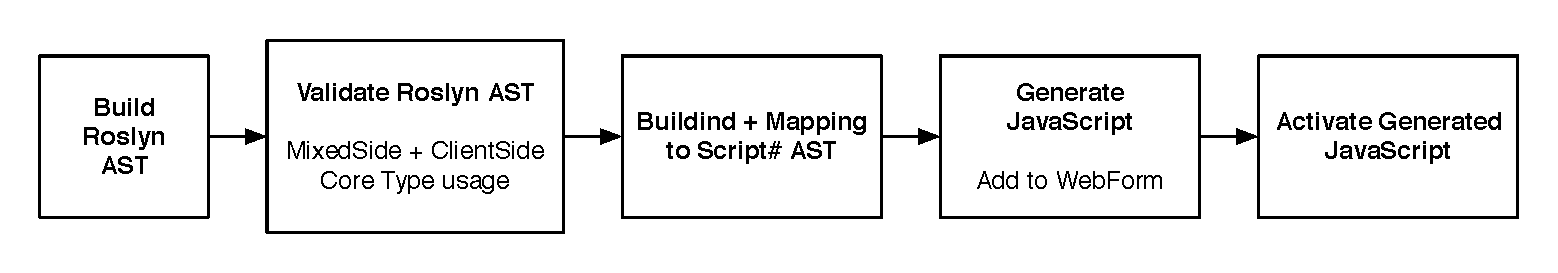
\includegraphics[width=14cm]{resources/images/internalworkflow.eps}}
	\end{center}
	\caption{The MiCS internal workflow}
	\label{fig:mics_internal_workflow}
\end{figure}

MiCS uses Roslyn to generate an Abstract Syntax Tree which is a syntatic representation of the user’s C\# code. Apart from the AST, a Semantic Model is generated to obtain information about what is being referenced.

When the Roslyn AST has been obtained it needs to be validated. This is done to ensure that the user uses types in a correct manner. Without validation, it would be possible for the user to generate non-working JavaScript.

Once the syntax tree has been validated, it is ready to be mapped to Script\#. This is the core functionality of MiCS - transforming a Roslyn AST to a Script\# AST. This step also ensures that the user does not utilize C\# constructs (declarations, statements and expressions) that we do not support. For example, at the moment the only supported loop-type is the for-loop. So if the user uses a while-loop or a foreach loop, the user gets an error telling them that an unsupported construct has been used.

When the Roslyn AST has successfully been mapped to Script\#, MiCS uses Script\#’s built-in ScriptGenerator to generate the JavaScript corresponding to the user’s original C\# code. 

When the JavaScript has been generated, it needs to be injected into the users WebForm. This is handled by a MiCSPage class; an extension to a WebForm Page. 

% section workflow_overview (end)

\section{Architecture} % (fold)
\label{sec:architecture}
Figure \ref{fig:dependencygraph} shows the most essential parts of the internal MiCS architecture and how the parts depend on each other. 
This section will describe the different parts, how they relate to one another and how the architecture relates to the five stages outlined in section \ref{sec:workflow_overview}. 

\begin{figure}
	\begin{center}
		\centerline{\includegraphics[width=18cm]{resources/images/dependencygraph.pdf}}
	\end{center}
	\caption{The most important parts of the MiCS architecture}
	\label{fig:dependencygraph}
\end{figure}


The TypeManagers (\texttt{TypeManager}, \texttt{CSharpTypeManager} and \texttt{ScriptSharpTypeManager}) provide information about types used throughout MiCS. For example, the TypeManagers are able to look up the type of a symbol (e.g. a variable). Furthermore, they can determine whether a given type is one that the user has defined, or if it is a built-in .NET-type.

The \texttt{Validator} class is responsible for validating the user's code in order to ensure correct type usage before the conversion to Script\# begins.

Classes in the Builders and Mappers namespaces serve as the backbone of MiCS. They are responsible for converting a Roslyn AST to its' corresponding Script\# AST. The Builders traverse the Roslyn AST and builds a corresponding Script\# AST, with help from the Mappers, that handle the actual conversion from Roslyn SyntaxNodes to the corresponding Script\# constructs. (Stage 3)

The \texttt{MiCSManager} class ties the entire MiCS project together and is involved in all of the stages described in section \ref{sec:workflow_overview}. It initializes all the ressource that MiCS needs to function (the TypeManagers) and subsequently initiates all of the processes needed to generate the JavaScript and inject it into the user's web page; first, it starts the validation of the user's code (stage 2). If the validation succeeds, the MiCSManager starts the conversion from Roslyn to Script\# by invoking the Builders (stage 3). When the Script\# AST has been generated, the MiCSManager uses Script\#'s \texttt{ScriptGenerator} to generate the JavaScript source code (stage 4). Lastly, the MiCSManager injects the generated JavaScript into the user's web page by using the pages registered \texttt{ScriptManager} (stage 5). 

% % section architecture (end)


\section{Detailed Scope}